\subsection{Analog simulations}

All simulations of the analog circuitry were done using the AimSpice SPICE backend~\cite{AIMSpice} along with the AIMPlot~\cite{aimplot} frontend.

The camera was simulated as a whole with the spice code described in Appendix~\ref{ap:SpiceCode} listing~\ref{lst:cameratoplevel}.
In order to show that the camera is working as intended it was simulated with 750 pA current from the diodes and 2 ms exposure time as well as 50 pA diode current and 30 ms as shown in figure~\ref{fig:analog7502}~and~\ref{fig:analog5030}.
This shows that the camera can handle both maximum and minimum lighting conditions without over or under exposure.

A more typical situation is shown in figure~\ref{fig:analog4003} with 400 pA diode current and 4 ms exposure.

The camera is still possible to overexpose as shown in figure~\ref{fig:analog40010}, the user should therefore set the exposure to a sensible level.

\begin{figure}[htbp]
  \centering
  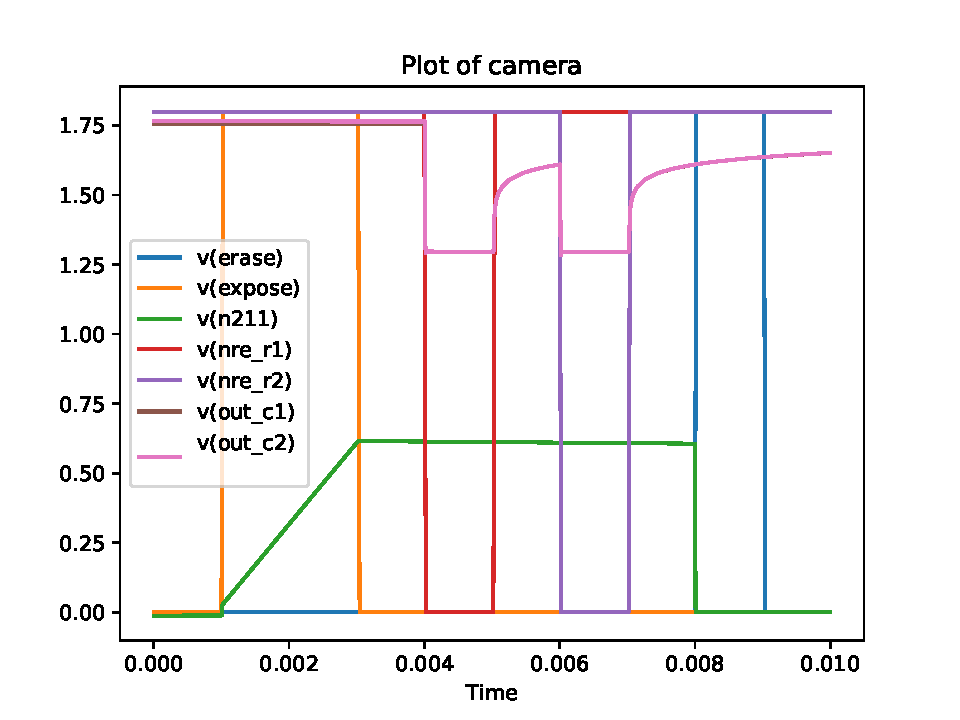
\includegraphics[width=0.75\textwidth]{../analog/camera7502}
  \caption{Analog camera tested with 750 pA and 2 ms}
  \label{fig:analog7502}
\end{figure}

\begin{figure}[htbp]
  \centering
  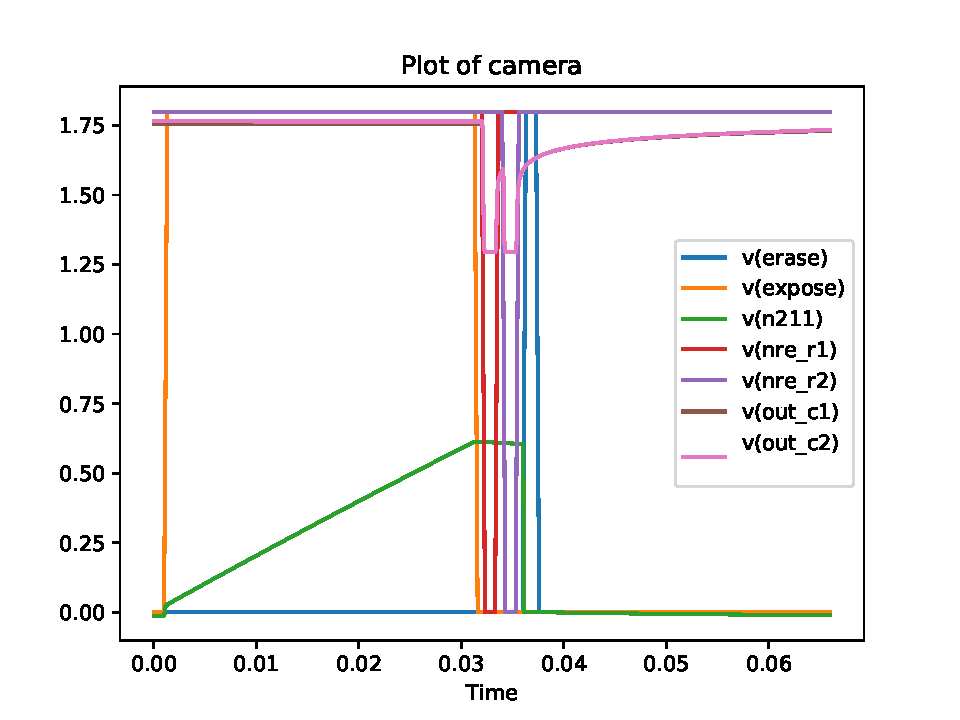
\includegraphics[width=0.75\textwidth]{../analog/camera5030}
  \caption{Analog camera tested with 50 pA and 30 ms}
  \label{fig:analog5030}
\end{figure}

\begin{figure}[htbp]
  \centering
  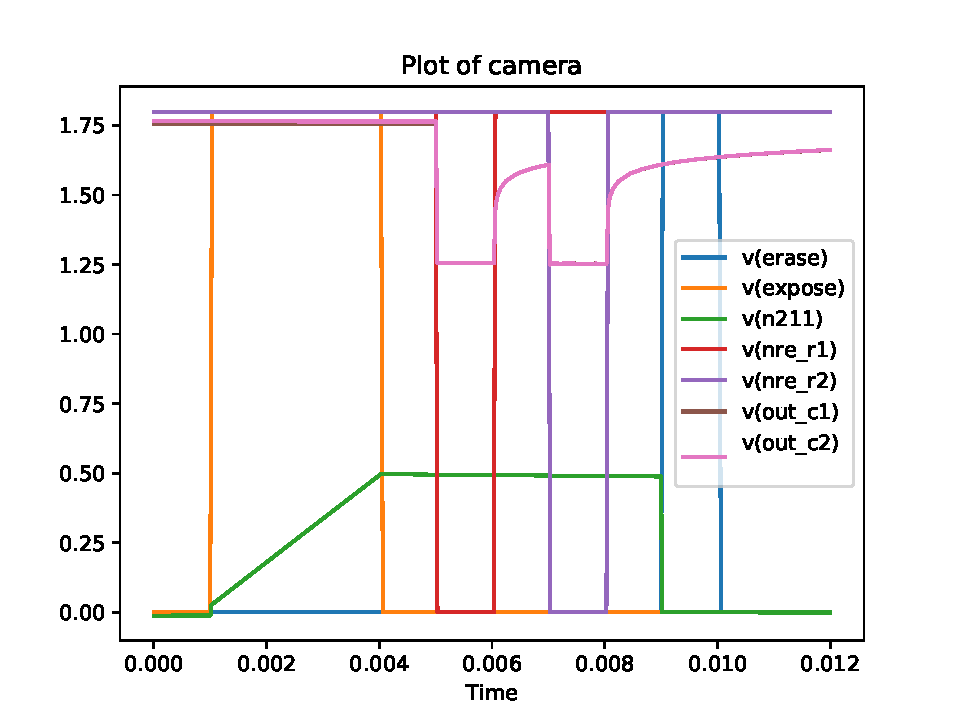
\includegraphics[width=0.75\textwidth]{../analog/camera4003typical}
  \caption{Analog camera tested with 400 pA and 3 ms}
  \label{fig:analog4003}
\end{figure}

\begin{figure}[htbp]
  \centering
  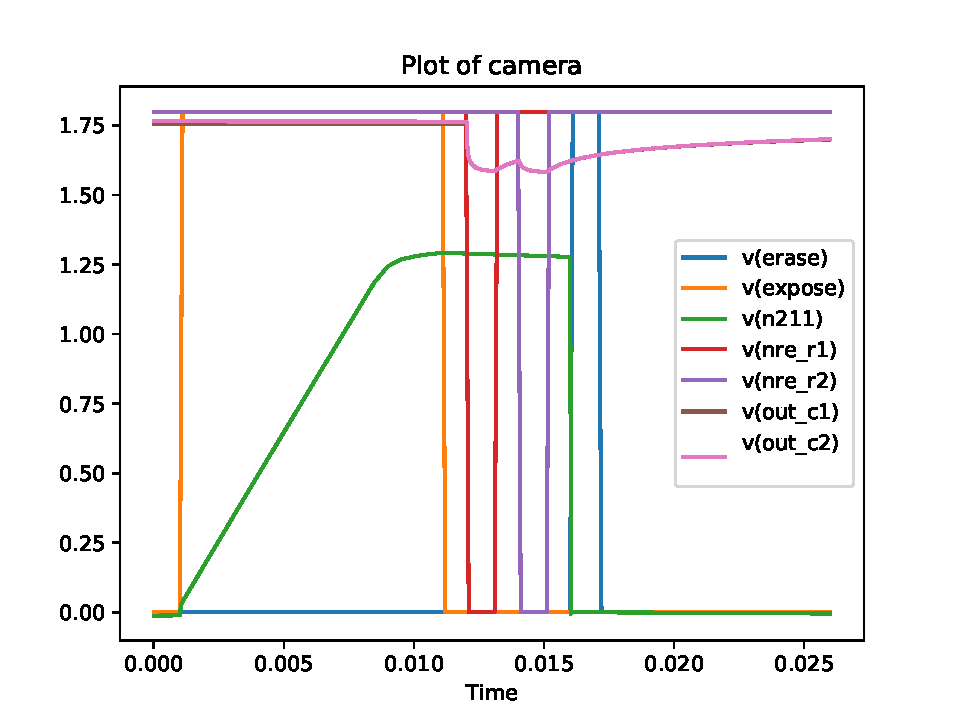
\includegraphics[width=0.75\textwidth]{../analog/camera40010overexposed}
  \caption{Analog camera tested with 400 pA and 10 ms}
  \label{fig:analog40010}
\end{figure}


Both the need for the current amplifiers and the possibility of leakage through M1 or M2 was discussed in Section~\ref{sec:AnalogDesign}.
In order to illustrate test these claims the camera was tested without the current amplifiers and with a leaky transistor M2 as shown in figures~\ref{fig:analog4003nocurrent}~and~\ref{fig:analogLeakingM2}.

\begin{figure}[htbp]
  \centering
  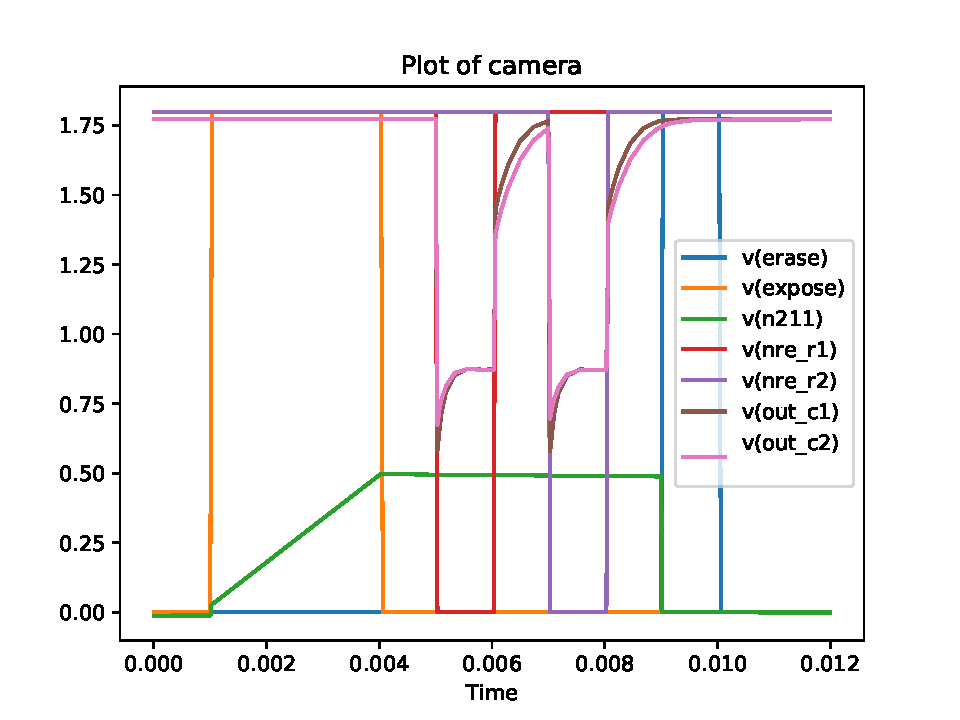
\includegraphics[width=0.75\textwidth]{../analog/camera4003nocurrentamp}
  \caption{Analog camera tested without current amplifiers}
  \label{fig:analog4003nocurrent}
\end{figure}

\begin{figure}[htbp]
  \centering
  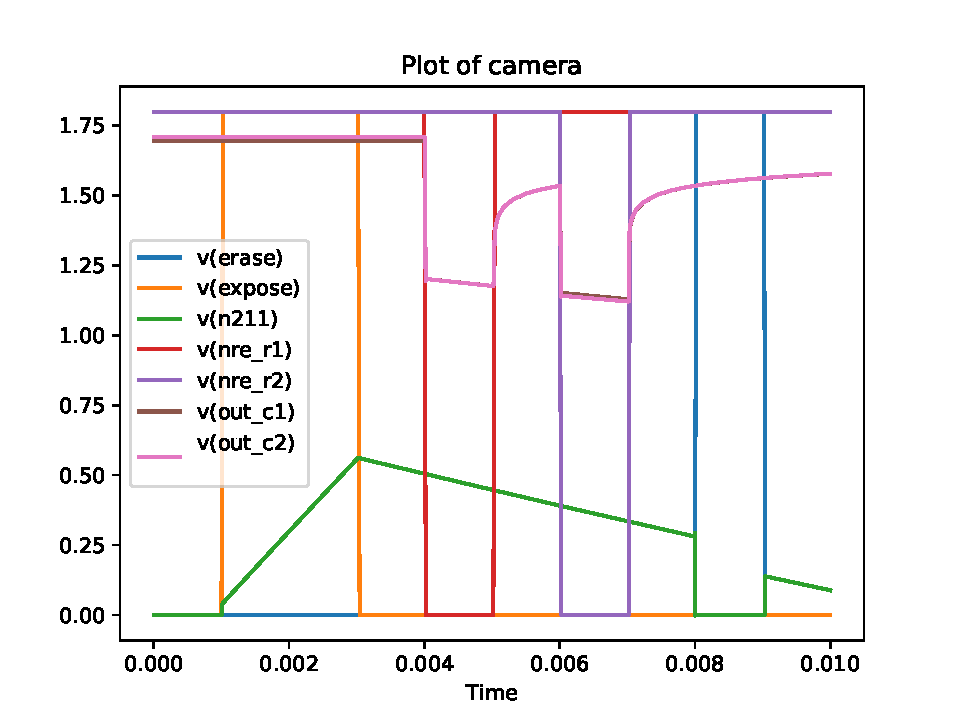
\includegraphics[width=0.75\textwidth]{../analog/cameraLeakingM2}
  \caption{Analog camera tested with transistor M2 tuned for maximum leakage}
  \label{fig:analogLeakingM2}
\end{figure}




\subsection{Digital simulations}

All simulation of the digital control system were run using SystemVerilog testbenches in icarus~verilog~\cite{icarusVL} and shown in GTKWave~\cite{gtkwave}.